\section{Introduction}
\label{sec:introduction}

Consider a puzzle about sorting,
inspired by Dijkstra's Dutch National Flag problem~\cite[Ch.14]{dijkstraDisciplineProgramming1997}.
Suppose there are balls of three colors,
corresponding to the colors of the Dutch flag: red, white, and blue.
\[
  \{
  \tikz[anchor=base, baseline]{%
    \foreach \x/\color in {1/red,2/white,3/blue} {
        \node[circle,draw,fill=\color,line width=1pt] at (\x,0) {\phantom{\tiny\x}};
        \ifthenelse{\NOT 1 = \x}{\node at ({\x-0.5},0) {,};}{}
      }
  }
  \}
\]
Given a finite multiset of such balls, how many ways can you sort them into the Dutch flag?
\[
  \{
      \tikz[anchor=base, baseline]{%
        \foreach \x/\color in {1/red,2/red,3/blue,4/white,5/blue,6/red,7/white,8/blue} {
            \node[circle,draw,fill=\color,line width=1pt] at (\x,0) {\phantom{\tiny\x}};
            \ifthenelse{\NOT 1 = \x}{\node at ({\x-0.5},0) {,};}{}
          }
      }
    \}
\]
Obviously there is only one way, which is given by the order
$\term{red} < \term{white} < \term{blue}$.
\[
  [
      \tikz[anchor=base, baseline]{%
        \foreach \x/\color in {1/red,2/red,3/red,4/white,5/white,6/blue,7/blue,8/blue} {
            \node[circle,draw,fill=\color,line width=1pt] at (\x,0) {\phantom{\tiny\x}};
            \ifthenelse{\NOT 1 = \x}{\node at ({\x-0.5},0) {,};}{}
          }
      }
    ]
\]

What if we are avid enjoyers of vexillology who also want to consider other flags?
We might ask: how many ways can we sort our finite multiset of balls?
We know that there are only $3! = 6$ permutations of
$\{\term{red}, \term{white}, \term{blue}\}$, so there are only 6 possible orderings we can define \footnote{We have no allegiance to any of the countries presented by the flags, hypothetical or otherwise. This is purely combinatorics!}.

\begin{center}
    \foreach \colorA/\colorB/\colorC in {red/white/blue, red/blue/white, white/red/blue, white/blue/red, blue/red/white, blue/white/red}{
    \begin{tikzpicture}[scale=0.5]
    \begin{flagdescription}{3/4}
    \hstripesIII{\colorA}{\colorB}{\colorC}
    \framecode{}
    \end{flagdescription}
    \end{tikzpicture}
    }
\end{center}

We posit that because there are exactly 6 orderings, we can only define 6 correct sorting
functions (up to function extensionality).

In more formal terms: let $A = \{\term{red}, \term{white}, \term{blue}\}$
let $\setord(A)$ be the set of orderings on $A$ and let 
 $\setmtol(A)$  be the set of functions $\term{FiniteMultiset}(A) \to \List(A)$.
There is a function $\otof : \setord(A) \to \setsort(A)$ that maps orderings to
some subset $\setsort(A) \subset \setmtol(A)$ which we call "sort functions":

\begin{center}
    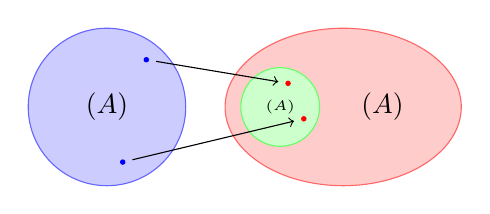
\begin{tikzpicture}
        % draw the sets
        \filldraw[fill=blue!20, draw=blue!60] (-1.5,0) circle (1cm);
        \filldraw[fill=red!20, draw=red!60] (1.5,0) ellipse (1.5cm and 1cm);
        \filldraw[fill=green!20, draw=green!60] (0.7,0) circle (0.5cm);
    
        % the texts
        \node at (-1.5,0) {$\Ord(A)$};
        \node at (0.7, 0) {\tiny$\Sort(A)$};
        \node at (2,0) {$\setmtol(A)$};

    
        % the points in the sets (here I just create nodes to use them later on to position
        % the circles and the arrows
        \node (x1) at (-1,0.6) {};
        \node (x2) at (-1.3,-0.7) {};
        \node (y1) at (0.8,0.3) {};
        \node (y2) at (1,-0.15) {};
    
        % position the elements in the sets (at the nodes we just created)
        \fill[blue] (x1) circle (1pt);
        \fill[blue] (x2) circle (1pt);
        \fill[red] (y1) circle (1pt);
        \fill[red] (y2) circle (1pt);
    
        % draw the arrows
        \draw[->] (x1) -- (y1);
        \draw[->] (x2) -- (y2);
    \end{tikzpicture}
\end{center}

This \textit{seems} trivial to prove: we can construct $\otof(r)$ by parameterizing
any sorting algorithm, e.g.\ insertion sort, by the order relation $r$ and we are done!
This however is not enough: we want to show that there are exactly 6 sorting functions because
there are exactly 6 orderings. In other words, $\setord(A)$ and $\setsort(A)$ should be
isomorphic. There should exist an inverse mapping to $\otof$ that allows us to construct
an ordering $\preccurlyeq$ given a function $s \in \setsort(A)$, such that
$\forall s \in \setsort(A).\, \otof(\otof^{-1}(s)) = s \land \forall r \in \setord(A).\, \otof^{-1}(\otof(r)) = r$.

To complete this proof formally we need to execute the following plan.
\begin{enumerate}
    \item We need to formalize exactly what $\term{FiniteMultiset}(A)$ and $\List(A)$ are.
    We formalize them in terms of universal algebra: $\term{FiniteMultiset}(A)$ is 
    the free commutative monoid on $A$ and $\List(A)$ is the free monoid on $A$. We give
    different constructions of them in~\cref{sec:monoids} and ~\cref{sec:commutative-monoids},
    proving these constructions correct by verifying their universal properties.
    We also explore the relationship between commutativity and ordering in
    ~\cref{sec:commutative-monoids} and ~\cref{sec:head},
    showing how imposing commutativity on a free monoid is same as "forgetting" the order.
    \item We need to nail down exactly what the subset $\Sort(A)$ is. In other words, we need to
    identify what properties functions $f \in \Sort(A) \subset \setmtol(A)$ satisfy which separate
    them from other functions $g \in \setmtol(A)$. We identify two properties in~\cref{sec:sorting},
    giving us two axioms for sorting functions which do not assume a pre-existing total order. This distinguishes our approach 
    from other formalizations of the correctness of sorting such as 
    \cite{appelVerifiedFunctionalAlgorithms2023}.
    \item Using the properties we have identified, we need to construct a full equivalence
    $\Sort(A) \simeq \Ord(A)$. Mapping orders to sorting functions is
    trivial by parameterizing insertion sort on an order relation. More interestingly we need to show how sorting functions
    can be mapped to orders, showing that the properties we have identified for $\Sort(A)$ indeed
    correctly identify the usual notion of soring functions.
\end{enumerate}

The term "formalize" in the above plan means exactly that, and we therefore need to choose a proof system in which to work. Martin-L\"of Type Theory (MLTT) would not be convenient because of the large amount of work with set quotients and commutativity in our theory. These concepts do not behave well in MLTT and often can only be modelled via setoids. While setoids would suffice for
our purposes, they carry a high proof burden which leads to a
phenomenon (un)affectionately named "setoid hell". We have therefore decided to formalize our proofs
for this paper in Cubical Agda~\cite{vezzosiCubicalAgdaDependently2019}. This allows us to work  naturally with
higher inductive types, and allows for a very simple method of transporting proofs between
different constructions of free algebras by univalence. What also makes Cubical Agda attractive
is that Cubical Type Theory allows us to enjoy the full power of univalence given by Homotopy Type Theory, 
without losing canonicity and computational content of the proofs. This means that proofs and functions
transported by univalence actually compute!
We give a table of our formalization in~\cref{sec:formalization}.

% MOVE SOME OF THESE TO DISCUSSION AND OTHER SECTIONS

% Intuitively, what should a correct sorting algorithm do?
% %
% All it knows about balls are their colors, so all it can do is compare balls by color, and move them around.
% %
% A correct sorting algorithm is going to rearrange these balls so the sequence gets partitioned into ``stripes''.
% \[
%   [
%       \tikz[anchor=base, baseline]{%
%         \foreach \x/\color in {1/red,2/red,3/red,4/white,5/white,6/blue,7/blue,8/blue} {
%             \node[circle,draw,fill=\color,line width=1pt] at (\x,0) {\phantom{\tiny\x}};
%             \ifthenelse{\NOT 1 = \x}{\node at ({\x-0.5},0) {,};}{}
%           }
%       }
%     ]
% \]
% There are 3 partitions corresponding to the 3 colors, hence there are $3! = 6$ ways to arrange the partitions.
% %
% Thus, the numbered of correct sorting functions is equal to the number of ways of ordering the colors!
% 
% \redtext{Intuition: what does a correct sorting algorithm do?}
% \begin{itemize}
%     \item It partitions the list by a key, in this case, the colors of the balls.
%     \item The keys need to be totally ordered in order to sort the partitions.
%     \item The number of total orderings will equal the number of possible ways of sorting the sequence.
% \end{itemize}
% \redtext{
%     We will use this simple observation as a motivation, but rather than thinking of it terms of counting, we will go a dimension higher and consider isomorphisms (or bijections) of sets. Is there a connection between the set of total orderings on the carrier set, and the set of correct sorting functions? Our discovery is that there is a bijection between the two! From this observation, we obtain an axiomatic understanding of the correctness of sorting.
% }
% 
% \subsection*{Solving the puzzle}
% 
% Suppose $A$ is the 3-element set $\{a,b,c\}$. There are many possible orderings of these elements,
% eg, $[a,b,c]$, or $[a,c,b]$, $[b,c,a]$, 6 of them.
% Consider lists of $A$, such as $[a,b,c,a,c,b,c,c]$, and we want to sort this list, so we want to write a sort function $s\colon List(A) \to List(A)$.
% Obviously, there would be infinitely many functions $\List(A) \to \List(A)$, but how many of them
% would actually be correct sorting functions? We posit that there are only 6 correct sorting
% functions, and our justification is because there are only 6 possible ordering on $A$.
% But how do we prove this?
% 
% Let's try to write some functions $\List(A) \to \List(A)$, for example:
% \begin{lstlisting}[language=haskell]
% s1 : List A $\to$ List A
% s1 [] = []
% s1 (x :: xs) = if x = a then ... else ...
% \end{lstlisting}
% $s1$ is a sort function only if $A$ is ordered by $a < c < b$.
% In fact, this goes both ways!
% If we write a correct sort function $s$, we will get a total order on $A$.
% We gain our main insight: fixing a permutation on $\{a,b,c\}$ fixes an ordering on the elements which determines a correct sort function for lists of $A$.
% 
% %% Now, suppose you have lists of elements of $A$, such as, $[(a,"foo"), (b, "bar"), (c, "baz")]$, and we want to sort this list using the first element of the tuple as the key -- in how many ways can we sort correctly?
% 
% %% Sorting algorithm is a common algorithm we introduce to undergraduate students
% %% when we teach them algorithmics. For example, a sort algorithm can be a function
% %% $\text{List} \, \mathbb{N} \to \text{List} \, \mathbb{N}$, which produces $[1,2,3,4]$
% %% given the input $[2,3,1,4]$.
% However, how do we formalize the correctness of this sort function?
% The common formalization of a correct sort algorithm is to say a sort algorithm produces
% an "orederd list", for example, one such formalization would be the definition
% from Verified Functional Algorithms \cite{appelVerifiedFunctionalAlgorithms2023}, translated into Agda.
% 
% \begin{lstlisting}[language=Haskell]
% data Sorted : List A $\to$ Type where
%   sorted-nil : Sorted []
%   sorted-one : $\forall$ x $\to$ Sorted [ x ]
%   sorted-cons : $\forall$ x y zs $\to$ x $\leq$ y $\to$ Sorted (y :: zs) $\to$ Sorted (x :: y :: zs)
% \end{lstlisting}
% 
% This is a perfectly valid formalization of an ordered list! Empty lists and singleton lists
% are ordered, and we can inductively construct an "orderness witness" by prepending a new element
% to an ordered list, provided that the new element is less than the head of the old ordered list of
% course. 
% 
% A correct sort function then has the type: \inline{sort : List A -> Sg(xs:List A).Sorted xs}.\vc{How is ours better?}
% This definition, however, assumes an existing total order on $A$. This is
% unsatisfactory, in a way, because a sorting algorithm is fundamentally just a function. Can we
% axiomatize the correctness of a sorting algorithm purely by the properties of functions?
% 
% % \begin{itemize}
% %     \item What exactly is special about commutativity? We study this from the ordinateur science point of view, using monoids and commutative monoids, which are important data structures.
% %     \item In some sense, commutativity or unordering is formally understood as non-determinism, such as in concurrency using finite powersets or free commutative monoids. When can a commutative structure be linearised?
% %     \item Commutativity is a way of enforcing unordering, or forgetting ordering, there are many ways of doing it: by using adjacent transpositions to generate all symmetries, or quotienting by symmetries
% %     \item if you forget the ordering and get an unordered list (or data structure), can you recover the ordering? Of course, it's a sorting algorithm, that is very basic to ordinateur science. In fact, this gives us a specification for sorting, which is our application.
% %     \item Why do we want to write intrinsically verified sorting algorithms?
% %         \begin{itemize}
% %         \item Using HITs, the sort function is correct by construction. This is unlike verifying
% %             sort externally in Coq.
% %         \item Can we structure the program in a better way? This is already solved by the bialgebraic sorting point of view, are we doing anything new?
% %         \item We give a more conceptual understanding of the correctness of sorting algorithms, using an abstract framework.
% %         \item Conventional way: a sort function turns a list into an ordered list.
% %         \item Our way: a sort function is a function satisfying some abstract properties, independent of a given ordering.
% %         \end{itemize}
% % \end{itemize}
% 
% % overall plan: with the universal algebra

% We can now study sorting from an algebraic perspective, viewing sorting as mappings from free commutative
% monoids to free monoids. There are many ways to construct free commutative monoids, such as using adjacent transpositions to generate all symmetries, or quotienting free monoids by symmetries, which we would
% elaborate on in ~\cref{sec:commutative-monoids}, all of which can be very naturally represented
% using higher inductive types in univalent type theory. We also
% create a framework for universal algebra, allowing us to formalize the notion of free algebras and
% their universal property, and finally within the framework we can formalize the axioms of sorting
% algorithms and their relationship to total orders.
% % Univalent type theory and Cubical Agda gives us a
% % rigorous framework for implementing these ideas, and higher inductive types allow us to express
% % the constructions of free commutative monoids very naturally.



\subsubsection*{Outline and Contributions}

\begin{myitemize}
  \item In~\cref{sec:type-theory}, we discuss the basics of HoTT and Cubical Agda, and describe the notation we use in the paper.
  \item In~\cref{sec:universal-algebra}, we give some background on a categorical framework for universal algebra including equations, and its formalization in HoTT. We give the definition of free algebras and their universal property.
  \item In~\cref{sec:monoids}, we give various constructions of free monoids, and their proofs of universal property.
  \item In~\cref{sec:commutative-monoids}, we add commutativity to free monoids, and show how to extend the proofs of universal property appropriately. Using our results we prove existing constructions
  of free commutative monoid are correct directly by their universal property, as opposed to
  the more common method of proving their correctness by isomorphism to known constructions
  of free commutative monoid.
  \item In~\cref{sec:combinatorics}, we show how free monoids and free commutative monoids are different, by discussing various combinatorial properties and operations, which can be defined for both, and ones which cannot be defined for both.
  \item In \cref{sec:sorting}, we build on the constructions of the previous sections and study intrinsically verified sorting function. The main result in this section is to connect total orders and sorting and commutativity, by proving an equivalence between decidable total orders on a carrier set $A$, and correct sorting algorithms on lists of elements of $A$.
  \item All the work in this paper is formalized in Cubical Agda, which is discussed in~\cref{sec:formalization}, and the accompanying code is available as supplementary material. Although the formalization is a contribution in itself, the purpose of the paper is not to discuss the formalization, but to present the results in un-formalized form, using HoTT/UF as a foundation, so the ideas are accessible to a wider audience, even without a background in type theory or formalization.
  \item In~\cref{sec:discussion}, we discuss connections to related work, and future work.
\end{myitemize}
